%&preformat-disser
\RequirePackage[l2tabu,orthodox]{nag} % Раскомментировав, можно в логе получать рекомендации относительно правильного использования пакетов и предупреждения об устаревших и нерекомендуемых пакетах
% Формат А4, 14pt (ГОСТ Р 7.0.11-2011, 5.3.6)
\documentclass[a4paper,14pt,oneside,openany]{memoir}

\input{common/setup}            % общие настройки шаблона
\input{common/packages}         % Пакеты общие для диссертации и автореферата
\synopsisfalse                      % Этот документ --- не автореферат
\input{Dissertation/dispackages}    % Пакеты для диссертации
\input{Dissertation/userpackages}   % Пакеты для специфических пользовательских задач

\input{Dissertation/setup}      % Упрощённые настройки шаблона

\input{common/newnames}         % Новые переменные, для всего проекта

\input{common/data}             % Основные сведения
\input{common/fonts}            % Определение шрифтов (частичное)
\input{common/styles}           % Стили общие для диссертации и автореферата
\input{Dissertation/disstyles}  % Стили для диссертации
\input{Dissertation/userstyles} % Стили для специфических пользовательских задач

%%% Библиография. Выбор движка для реализации %%%
% Здесь только проверка установленного ключа. Сама настройка выбора движка
% размещена в common/setup.tex
\ifnumequal{\value{bibliosel}}{0}{%
    \input{biblio/predefined}   % Встроенная реализация с загрузкой файла через движок bibtex8
}{
    \input{biblio/biblatex}     % Реализация пакетом biblatex через движок biber
}

% Вывести информацию о выбранных опциях в лог сборки
\typeout{Selected options:}
\typeout{Draft mode: \arabic{draft}}
\typeout{Font: \arabic{fontfamily}}
\typeout{AltFont: \arabic{usealtfont}}
\typeout{Bibliography backend: \arabic{bibliosel}}
\typeout{Precompile images: \arabic{imgprecompile}}
% Вывести информацию о версиях используемых библиотек в лог сборки
\listfiles

%%% Управление компиляцией отдельных частей диссертации %%%
% Необходимо сначала иметь полностью скомпилированный документ, чтобы все
% промежуточные файлы были в наличии
% Затем, для вывода отдельных частей можно воспользоваться командой \includeonly
% Ниже примеры использования команды:
%
%\includeonly{Dissertation/part2}
%\includeonly{Dissertation/contents,Dissertation/appendix,Dissertation/conclusion}
%
% Если все команды закомментированы, то документ будет выведен в PDF файл полностью

\begin{document}
%%% Переопределение именований типовых разделов
% https://tex.stackexchange.com/a/156050
\gappto\captionsrussian{\input{common/renames}\unskip} % for polyglossia and babel
\input{common/renames}

%%% Структура диссертации (ГОСТ Р 7.0.11-2011, 4)
%\include{Dissertation/title}           % Титульный лист
\include{Dissertation/contents}        % Оглавление
\chapter*{Реферат}
\addcontentsline{toc}{chapter}{Реферат} 
\section*{Актуальность темы}
\noindent Текст, первый абзац без отступа. Реферат схож с аннотацией к научной статье, но должна быть более детальной

Следующий абзац с отступом. Кратко повторите основное содержание диссертации, включая мотивацию для этой работы, новизну по сравнению с предыдущими работами, описание проблемы, методологию, результаты и выводы.
\section*{Научная новизна}
\section*{Научные положения, выносимые на защиту:}
\section*{Практическая значимость}
\section*{Достоверность}
\section*{Внедрение результатов работы}
\section*{Публикации}
\section*{Личный вклад автора}
\section*{Структура и объем диссертации}
\section*{ОСНОВНОЕ СОДЕРЖАНИЕ РАБОТЫ}
\chapter*{Synopsis}
\addcontentsline{toc}{chapter}{Synopsis} 
\section*{Relevance}
\noindent Текст, первый абзац без отступа. Реферат схож с аннотацией к научной статье, но должна быть более детальной

Следующий абзац с отступом. Кратко повторите основное содержание диссертации, включая мотивацию для этой работы, новизну по сравнению с предыдущими работами, описание проблемы, методологию, результаты и выводы.
\section*{The goal}
\section*{Scientific tasks:}
\section*{Scientific novelty}
\section*{Scientific statements:}
\section*{Practical importance}
\section*{Reliability and the validity}
\section*{Implementation of the obtained results}
\section*{Approbation}
\section*{Publication}
\section*{Author contribution}
\section*{The structure}
\section*{MAIN CONTENTS OF WORK}
\ifnumequal{\value{contnumfig}}{1}{}{\counterwithout{figure}{chapter}}
\ifnumequal{\value{contnumtab}}{1}{}{\counterwithout{table}{chapter}}
\chapter*{Введение}                         % Заголовок
\addcontentsline{toc}{chapter}{Введение}    % Добавляем его в оглавление

\newcommand{\actuality}{}
\newcommand{\progress}{}
\newcommand{\aim}{{\textbf\aimTXT}}
\newcommand{\tasks}{\textbf{\tasksTXT}}
\newcommand{\novelty}{\textbf{\noveltyTXT}}
\newcommand{\influence}{\textbf{\influenceTXT}}
\newcommand{\methods}{\textbf{\methodsTXT}}
\newcommand{\defpositions}{\textbf{\defpositionsTXT}}
\newcommand{\reliability}{\textbf{\reliabilityTXT}}
\newcommand{\probation}{\textbf{\probationTXT}}
\newcommand{\contribution}{\textbf{\contributionTXT}}
\newcommand{\publications}{\textbf{\publicationsTXT}}


{\actuality} 


\ifsynopsis
Этот абзац появляется только в~автореферате.
Для формирования блоков, которые будут обрабатываться только в~автореферате,
заведена проверка условия \verb!\!\verb!ifsynopsis!.
Значение условия задаётся в~основном файле документа (\verb!synopsis.tex! для
автореферата).
\else
Этот абзац появляется только в~диссертации.
Через проверку условия \verb!\!\verb!ifsynopsis!, задаваемого в~основном файле
документа (\verb!dissertation.tex! для диссертации), можно сделать новую
команду, обеспечивающую появление цитаты в~диссертации, но~не~в~автореферате.
\fi

% {\progress}
% Этот раздел должен быть отдельным структурным элементом по
% ГОСТ, но он, как правило, включается в описание актуальности
% темы. Нужен он отдельным структурынм элемементом или нет ---
% смотрите другие диссертации вашего совета, скорее всего не нужен.

{\aim} данной работы является \ldots

Для~достижения поставленной цели необходимо было решить следующие {\tasks}:
\begin{enumerate}[beginpenalty=10000] % https://tex.stackexchange.com/a/476052/104425
  \item Исследовать, разработать, вычислить и~т.\:д. и~т.\:п.
  \item Исследовать, разработать, вычислить и~т.\:д. и~т.\:п.
  \item Исследовать, разработать, вычислить и~т.\:д. и~т.\:п.
  \item Исследовать, разработать, вычислить и~т.\:д. и~т.\:п.
\end{enumerate}


{\novelty}
\begin{enumerate}[beginpenalty=10000] % https://tex.stackexchange.com/a/476052/104425
  \item Впервые \ldots
  \item Впервые \ldots
  \item Было выполнено оригинальное исследование \ldots
\end{enumerate}

{\influence} \ldots

{\methods} \ldots

{\defpositions}
\begin{enumerate}[beginpenalty=10000] % https://tex.stackexchange.com/a/476052/104425
  \item Первое положение
  \item Второе положение
  \item Третье положение
  \item Четвертое положение
\end{enumerate}
В папке Documents можно ознакомиться в решением совета из Томского ГУ
в~файле \verb+Def_positions.pdf+, где обоснованно даются рекомендации
по~формулировкам защищаемых положений.

{\reliability} полученных результатов обеспечивается \ldots \ Результаты находятся в соответствии с результатами, полученными другими авторами.


{\probation}
Основные результаты работы докладывались~на:
перечисление основных конференций, симпозиумов и~т.\:п.

{\contribution} Автор принимал активное участие \ldots

\ifnumequal{\value{bibliosel}}{0}
{%%% Встроенная реализация с загрузкой файла через движок bibtex8. (При желании, внутри можно использовать обычные ссылки, наподобие `\cite{vakbib1,vakbib2}`).
    {\publications} Основные результаты по теме диссертации изложены
    в~XX~печатных изданиях,
    X из которых изданы в журналах, рекомендованных ВАК,
    X "--- в тезисах докладов.
}%
{%%% Реализация пакетом biblatex через движок biber
    \begin{refsection}[bl-author, bl-registered]
        % Это refsection=1.
        % Процитированные здесь работы:
        %  * подсчитываются, для автоматического составления фразы "Основные результаты ..."
        %  * попадают в авторскую библиографию, при usefootcite==0 и стиле `\insertbiblioauthor` или `\insertbiblioauthorgrouped`
        %  * нумеруются там в зависимости от порядка команд `\printbibliography` в этом разделе.
        %  * при использовании `\insertbiblioauthorgrouped`, порядок команд `\printbibliography` в нём должен быть тем же (см. biblio/biblatex.tex)
        %
        % Невидимый библиографический список для подсчёта количества публикаций:
        \printbibliography[heading=nobibheading, section=1, env=countauthorvak,          keyword=biblioauthorvak]%
        \printbibliography[heading=nobibheading, section=1, env=countauthorwos,          keyword=biblioauthorwos]%
        \printbibliography[heading=nobibheading, section=1, env=countauthorscopus,       keyword=biblioauthorscopus]%
        \printbibliography[heading=nobibheading, section=1, env=countauthorconf,         keyword=biblioauthorconf]%
        \printbibliography[heading=nobibheading, section=1, env=countauthorother,        keyword=biblioauthorother]%
        \printbibliography[heading=nobibheading, section=1, env=countregistered,         keyword=biblioregistered]%
        \printbibliography[heading=nobibheading, section=1, env=countauthorpatent,       keyword=biblioauthorpatent]%
        \printbibliography[heading=nobibheading, section=1, env=countauthorprogram,      keyword=biblioauthorprogram]%
        \printbibliography[heading=nobibheading, section=1, env=countauthor,             keyword=biblioauthor]%
        \printbibliography[heading=nobibheading, section=1, env=countauthorvakscopuswos, filter=vakscopuswos]%
        \printbibliography[heading=nobibheading, section=1, env=countauthorscopuswos,    filter=scopuswos]%
        %
        \nocite{*}%
        %
        {\publications} Основные результаты по теме диссертации изложены в~\arabic{citeauthor}~печатных изданиях,
        \arabic{citeauthorvak} из которых изданы в журналах, рекомендованных ВАК\sloppy%
        \ifnum \value{citeauthorscopuswos}>0%
            , \arabic{citeauthorscopuswos} "--- в~периодических научных журналах, индексируемых Web of~Science и Scopus\sloppy%
        \fi%
        \ifnum \value{citeauthorconf}>0%
            , \arabic{citeauthorconf} "--- в~тезисах докладов.
        \else%
            .
        \fi%
        \ifnum \value{citeregistered}=1%
            \ifnum \value{citeauthorpatent}=1%
                Зарегистрирован \arabic{citeauthorpatent} патент.
            \fi%
            \ifnum \value{citeauthorprogram}=1%
                Зарегистрирована \arabic{citeauthorprogram} программа для ЭВМ.
            \fi%
        \fi%
        \ifnum \value{citeregistered}>1%
            Зарегистрированы\ %
            \ifnum \value{citeauthorpatent}>0%
            \formbytotal{citeauthorpatent}{патент}{}{а}{}\sloppy%
            \ifnum \value{citeauthorprogram}=0 . \else \ и~\fi%
            \fi%
            \ifnum \value{citeauthorprogram}>0%
            \formbytotal{citeauthorprogram}{программ}{а}{ы}{} для ЭВМ.
            \fi%
        \fi%
        % К публикациям, в которых излагаются основные научные результаты диссертации на соискание учёной
        % степени, в рецензируемых изданиях приравниваются патенты на изобретения, патенты (свидетельства) на
        % полезную модель, патенты на промышленный образец, патенты на селекционные достижения, свидетельства
        % на программу для электронных вычислительных машин, базу данных, топологию интегральных микросхем,
        % зарегистрированные в установленном порядке.(в ред. Постановления Правительства РФ от 21.04.2016 N 335)
    \end{refsection}%
    \begin{refsection}[bl-author, bl-registered]
        % Это refsection=2.
        % Процитированные здесь работы:
        %  * попадают в авторскую библиографию, при usefootcite==0 и стиле `\insertbiblioauthorimportant`.
        %  * ни на что не влияют в противном случае
        \nocite{vakbib2}%vak
        \nocite{patbib1}%patent
        \nocite{progbib1}%program
        \nocite{bib1}%other
        \nocite{confbib1}%conf
    \end{refsection}%
        %
        % Всё, что вне этих двух refsection, это refsection=0,
        %  * для диссертации - это нормальные ссылки, попадающие в обычную библиографию
        %  * для автореферата:
        %     * при usefootcite==0, ссылка корректно сработает только для источника из `external.bib`. Для своих работ --- напечатает "[0]" (и даже Warning не вылезет).
        %     * при usefootcite==1, ссылка сработает нормально. В авторской библиографии будут только процитированные в refsection=0 работы.
}


 % Характеристика работы по структуре во введении и в автореферате не отличается (ГОСТ Р 7.0.11, пункты 5.3.1 и 9.2.1), потому её загружаем из одного и того же внешнего файла, предварительно задав форму выделения некоторым параметрам

\textbf{Объем и структура работы.} Диссертация состоит из~введения,
\formbytotal{totalchapter}{глав}{ы}{}{},
заключения и
\formbytotal{totalappendix}{приложен}{ия}{ий}{}.
%% на случай ошибок оставляю исходный кусок на месте, закомментированным
%Полный объём диссертации составляет  \ref*{TotPages}~страницу
%с~\totalfigures{}~рисунками и~\totaltables{}~таблицами. Список литературы
%содержит \total{citenum}~наименований.
%
Полный объём диссертации составляет
\formbytotal{TotPages}{страниц}{у}{ы}{}, включая
\formbytotal{totalcount@figure}{рисун}{ок}{ка}{ков} и
\formbytotal{totalcount@table}{таблиц}{у}{ы}{}.
Список литературы содержит
\formbytotal{citenum}{наименован}{ие}{ия}{ий}.

\begin{tabular}{l|c|c}
Система & Эксперименты & Расчеты \\
%\hline
Графен / Fe / Ni(111) & - & + \\
Графен / Fe$_3$Si / Ni(111) & - & + \\
Графен / Co / Ni(111) & +* & + \\
Графен / Co$_3$Si / Ni(111) & + & + \\
Графен / Fe / SiC (0001) & + & + \\
Графен / Fe$_3$Si / SiC (0001) & + & + \\
Графен / Co / SiC (0001) & + & + \\
Графен / Co$_3$Si / SiC (0001) & + & + \\
Co$_2$FeSi & -** & + \\
\hline

\end{tabular}

* Тут я сама в экспериментах не участвовала, но обрабатывала некоторые результаты и включена в число соавторов статьи по теме.

** Эксперименты должны быть проведены когда-то на Бесси (пока даты назначены в июне)    % Введение
\ifnumequal{\value{contnumfig}}{1}{\counterwithout{figure}{chapter}
}{\counterwithin{figure}{chapter}}
\ifnumequal{\value{contnumtab}}{1}{\counterwithout{table}{chapter}
}{\counterwithin{table}{chapter}}
%\include{Dissertation/part1}           % Глава 1
%\include{Dissertation/part2}           % Глава 2
%\include{Dissertation/part3}           % Глава 3
\chapter{ Обзор литературы} \label{chapt1}
\section{ Графен}
Углерод является одним из самых распространенных веществ на Земле.  Он является частью огромного числа органических соединений, а также способен образовывать различные кристаллические структуры, такие как графит, алмаз, фуллерены и так далее. Такое разнообразие обусловлено особенностями электронной структуры углерода. В основном состоянии он находится в конфигурации $1s^22s^22p^2$.  При образовании ковалентной связи углерод переходит в возбужденное состояние $1s^22s^12p^3$. Повышение энергии при этом является оправданным, так как приводит к повышению энергии связи углерода с соседями.

	Для атома углерода возможны различные варианты гибридизации $s$  и $p$ орбиталей. Так, $sp^3$  гибридизация приводит к образованию алмаза, $sp^2$ гибридизация характерна для графита, а $sp$ гибридизация — для карбина.
	В случае смешения одной  $s$ и двух $p$ волновых функций образуются 3 гибридные  $sp^2$ орбитали, лежащие в одной плоскости. Они участвуют в образовании $\sigma$ связей. Оставшаяся $p_z$ орбиталь располагается перпендикулярно $sp^2$ плоскости и принимает участие в образовании  $\pi$ связи. Именно  $sp^2$ гибридизация ответственна за формирование графена. Графен — это двумерный материал, представляющий собой моноатомный слой углерода, обладающий сотовой структурой.
 \begin{figure}[ht] 
  \center
  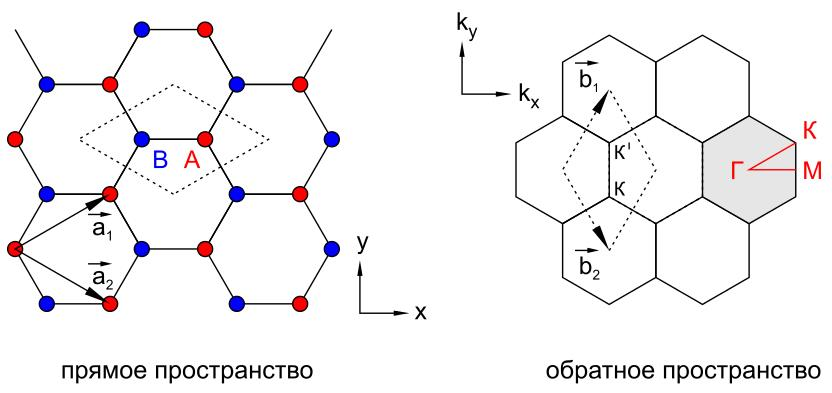
\includegraphics [scale=0.47] {11}
  \caption{Решётка графена в прямом и обратном пространстве.} 
  \label{img:11}  
\end{figure}

	Элементарная ячейка графена состоит из двух неэквивалентных атомов, образующих две подрешетки (Рис.\ref{img:11}). Используя вектора трансляции, невозможно получить одну подрешетку из другой. С другой стороны, атомы разных подрешеток имеют одинаковое окружение и являются в этом смысле эквивалентными. Постоянная решетки равна 2.46 Å, расстояние между двумя ближайшими атомами 1.42 Å. Обратная решетка также является сотовой структурой, форма первой зоны Бриллюэна — шестиугольник (Рис.\ref{img:11}).\cite{0953-8984-29-46-465901}
	
	Первые расчеты электронной структуры графена были проведены в 1947 году в приближении сильной связи \cite{1}. Четыре валентные орбитали каждого атома участвуют в образовании трех $\sigma$ и одной $\pi$ связи. При этом особый интерес представляет дисперсия $\pi$ состояний. Зонная структура графена представлена на Рис.\ref{img:12}.
 \begin{figure}[ht] 
  \center
  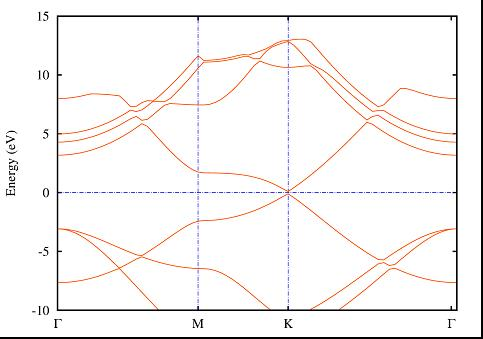
\includegraphics [scale=0.77] {12}
  \caption{Зонная структура графена, построенная вдоль высокосимметричных направлений первой зоны Бриллюэна.} 
  \label{img:12}  
\end{figure}

	Главной особенностью электронной структуры графена является наличие линейной дисперсии $\pi$-состояний вблизи точки К. Оба атома элементарной ячейки отдают по электрону для формирования  зон, вследствие чего связывающая $\pi$ орбиталь оказывается полностью заполненной, а разрыхляющая $\pi*$ орбиталь полностью пустой.  В точке К на уровне Ферми заполненный и незаполненный конус касаются друг друга. Наблюдается вырождение валентной зоны и зоны проводимости. Поэтому графен относят к бесщелевым полупроводникам. Коническая поверхность $E(k)$ вблизи точки К называется конусом Дирака. 
	
	Графен механически прочен, химически стоек и обладает рекордно высокой подвижностью носителей заряда. В силу выдающихся свойств он является чрезвычайно привлекательным для применений в электронике \cite{2}
\section{ Графен на подложке} \label{chapt_graphene-sic}
Линейный закон дисперсии вблизи точек касания валентной зоны и зоны проводимости присущ идеальному графену. В реальности графен всегда находится на подложке, с которой взаимодействует. Возникающие при этом модификации свойств графена являются следствием физико-химических свойств материала подложки. Для того чтобы научиться контролируемо модифицировать свойства графена, важно понимать, как именно происходит взаимодействие графена и вещества, на котором он находится. 

Для синтеза графена на металлических подложках широко используется метод химического осаждения из газовой фазы (CVD). Плотноупакованные грани Ni(111) и Co(0001) имеют постоянные решетки, близкие к постоянной решетки графена, что позволяет осуществлять рост высококачественного графена большой площади и делает эти интерфейсы удобными объектами исследования. Помимо этих двух металлов, графен может быть успешно синтезирован на Cu, Ir, Ru, Rh и Au. Дальнейшая модификация свойств графена может быть проведена с использованием процесса интеркаляции, который описан в следующем разделе.

	Наибольшее внимание уделялось системе графен/Ni(111) \cite{3,4,5,6,7,8,9,10}, что в значительной степени обусловлено возможностью формирования высококачественного графена на никеле методом химического осаждения из газовой фазы. В силу почти идеального соответствия постоянных решетки графена и никеля (отличие составляет менее 1,5 процентов) образуется плоская структура $p$(1 x 1) \cite{3}. 


	Экспериментальное и теоретическое исследование графена на никеле показало, что наличие подложки оказывает существенное влияние на его электронную структуру. По сравнению со структурой графита она сдвинута в сторону бÓльших энергий связи на 3 eV. Это обусловлено гибридизацией 3d состояний Ni с $p_z$ состояниями графена \cite{6}. Показано также, что вследствие сильного взаимодействия графена с металлической подложкой происходит значительная модификация электронной структуры графена и разрушение линейной дисперсионной зависимости $p_z$ состояний графена вблизи точки K зоны Бриллюэна. Перекрытие $\pi$ орбиталей углерода с $3d$ орбиталями никеля по энергии и в прямом и обратном пространстве приводит к тому, что в окрестности точки К зоны Бриллюэна появляется несколько гибридных состояний. Образующиеся гибридные орбитали обладают различной симметрией, и поэтому вырождение в точке К снимается через образование зазора. 
	
	
	Общий подход к пониманию электронной структуры графена на металлической подложке предложен в работе \cite{9}. В случае адсорбции графена на sp-металлах sp-электроны металла заполняют конус Дирака, что ведет к его смещению в область больших энергий связи и n-допированию графена.  Величина этого смещения, а также равновесное расстояние между графеном и подложкой зависит от разности работ выхода металла и графена. При этом линейная дисперсия $\pi$-состояний углерода остается ненарушенной. 
	
	Иная ситуация реализуется в случае взаимодействия графена с металлами с незаполненной 3d оболочкой. При перестройке электронной структуры графена происходят два процесса. Сначала, как и при взаимодействии с sp-металлами, конус Дирака смещается вследствие его заполнения sp-электронами подложки. В результате $\pi$-состояния углерода начинают перекрываться с 3d состояниями металла по шкале энергий. Вследствие этого происходит гибридизация этих состояний, и, следовательно, разрушение линейной дисперсии $\pi$-состояний вблизи точки К. 
\begin{figure}[ht] 
  \center
  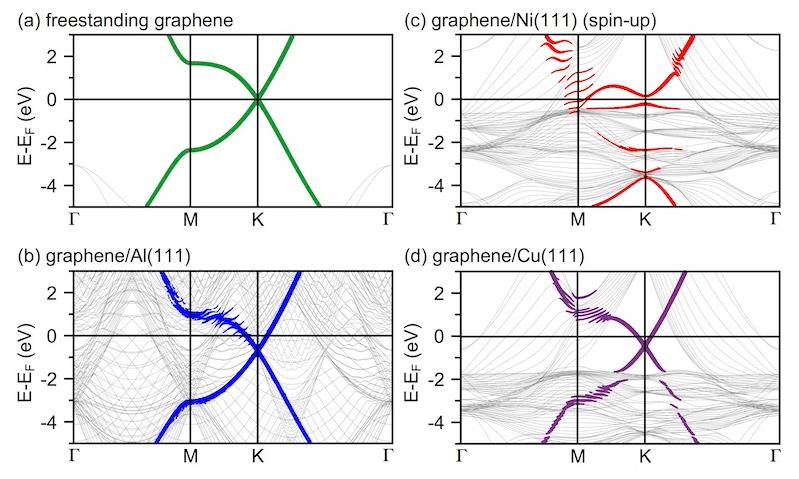
\includegraphics [scale=0.67] {25}
  \caption{Электронная структура свободного графена (a), электронная структура систем графен/Al(111) (b), графен/Ni(111) (с), графен/Сu(111) (d)  \cite{10}.} 
  \label{img:25}  
\end{figure}
	Выводы, сделанные для адсорбции графена на sp-металлах и металлах с незакрытой d-оболочкой, могут быть обобщены на случай взаимодействия графена с металлом с закрытой d-оболочкой.  Начальное допирование графена обусловлено sp-электронами металла. Заполненная d-оболочка оказывается расположена ниже точки Дирака, поэтому образование гибридных орбиталей в местах перекрытия $\pi$-состояний углерода и d-состояний металла не затрагивает конус Дирака.
	
	Приведенные рассуждения проиллюстрированы на Рис.\ref{img:25}. Зонная структура свободного графена показана на Рис. \ref{img:25} а. Энергетическая структура системы графен/Al(111), рассчитанная из первых принципов, приведена на Рис. \ref{img:25} b. Вклад $\pi$-состояний углерода выделен  синим цветом. Видно, что энергетическая структура $\pi$-состояний фактически повторяет дисперсионную характеристику свободнолежащего графена. Зонная структура системы графен/Ni(111) значительно видоизменена по сравнению с предыдущим случаем (Рис. \ref{img:25} c): из-за гибридизации линейная дисперсия $\pi$-состояний нарушается, и образуется несколько гибридных состояний. Наконец, энергетическая структура системы графен/Cu(111) показана на Рис. \ref{img:25} d. Видно, что в этом случае гибридизация не затрагивает конус Дирака в точке К. 
	
Другим популярным методом синтеза графена является термическое разложение карбида кремния. Данный способ позволяет получать высококачественный графен большой площади \cite{Davydov2017} на диэлектрической подложке. 
\begin{figure}[ht] 
  \center
  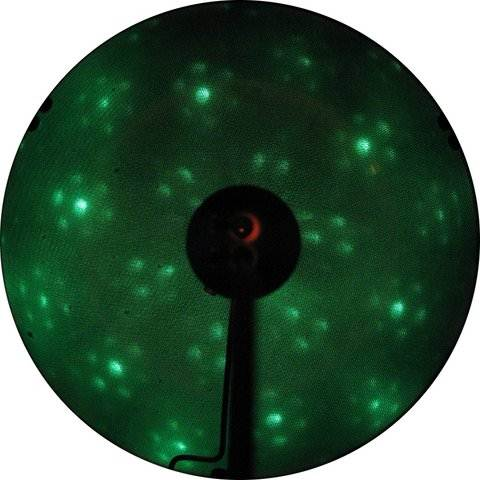
\includegraphics [scale=0.67] {gr-sic-leed}
  \caption{Картина дифракции медленных электронов для системы графен/SiC(0001)} 
  \label{img:leed_sic}  
\end{figure}
При этом между графеном и подложкой образуется буферный слой, представляющий собой графеноподобный слой атомов углерода, связанный с атомами кремния подложки. Расстояние между атомами буферного слоя и атомами кремния изменяется от 1.98Å до 2.25Å   А. В то же время расстояние между графеном и буферным слоем оказывается сравнимым с межплоскостным расстоянием в графите и составляет 3.15Å. В силу несоответствия постоянных решетки карбида кремния и графена возникает суперструктура $p(6\sqrt{3}\times6\sqrt{3})R30^{\circ}$, соответствующая наложению 169 ячеек графена на 108 ячеек подложки. Данная суперструктура проявляется как на картинах дифракции медленных электронов (Рис. \ref{img:leed_sic}), так и на на изображениях, снятых с помощью сканирующего туннельного микроскопа \cite{ab_initio_stm}.
\begin{figure}[ht] 
  \center
  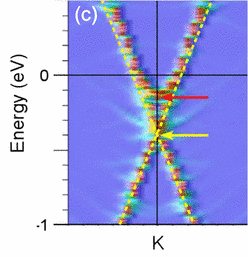
\includegraphics [scale=1] {gr-sic-dft}
  \caption{Фрагмент расчета зонной структуры системы графен/SiC(0001) из работы \cite{PhysRevLett.105.085502}.} 
  \label{img:gr-sic-dft}  
\end{figure}
Электронная структура графена в этом случае также оказывается изменена по сравнению со случаем свободного графена без подложки: конус Дирака смещается на 0.45 eV в сторону больших энергий связи, а состояния атомов углерода буферного слоя расположены на несколько электронвольт ниже уровня Ферми, что говорит о сильной связи этих атомов с атомами кремния \cite{AGRAWAL2013102}.
Наличие буферного слоя обуславливает основной недостаток графена, сформированного на карбиде кремния: рассеяние электронов на атомах буферного слоя ухудшает его транспортные свойства.




	
\section{ Интеркаляция графена} \label{chapt3}
Одним из перспективных способов целенаправленного изменения электронных и магнитных свойств интерфейса графен/подложка является интеркаляция его атомами или молекулами других веществ, т.е. внедрение инородных частиц под графен. Для активации процесса интеркаляции, как правило, необходим отжиг предварительно нанесенной на графен пленки инородного вещества. К настоящему времени имеется целый ряд работ, демонстрирующих большой потенциал данного способа модификации графена. Так, например, показано, что интеркаляция графена благородными металлами \cite{10,11} или атомами водорода \cite{12} может быть использована для уменьшения взаимодействия между графеном и подложкой, вплоть до восстановления электронных свойств свободного графена. В то же время интеркаляция  щелочными металлами является  эффективным средством управления уровнем электронного допирования графена \cite{13}. Наконец, интеркаляция графена атомами ферромагнитных металлов может приводить к появлению у него магнитных свойств \cite{8}. Этот способ также весьма перспективен для изготовления структур типа графен/ферромагнитный металл, обладающих перпендикулярной магнитной анизотропией \cite{14,15,16}. Ввиду того, что такие структуры представляют большой научный и практический интерес, графен, сформированный на поверхности магнитных металлов стал объектом активных исследований в последние годы.
\begin{figure}[ht] 
  \center
  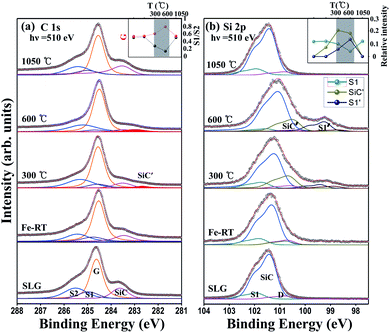
\includegraphics [scale=1] {c1s}
  \caption{Спектры С $1s$ и Si $2p$, полученные при различных температурах отжига в работе \cite{C3NR04178F}}. 
  \label{img:c1s}  
\end{figure}

	Влияние интеркаляции железа на атомное строение, электронную структуру и магнитные свойства интерфейса графен/Ni(111) исследовалось в работах \cite{17,18}.  Атомная структура и электронное строение интеркалированных слоев железа исследованы в работе \cite{19}, авторы которой использовали методы ДМЭ и рентгеновской ФЭС, а также провели теоретические расчеты, выполненные из первых принципов. Установлено, что пленки железа толщиной в один и два монослоя имеют такую же ГЦК структуру, как и подложка Ni(111), а атомы углерода располагаются над атомами железа в тех же местах, что и над атомами никелевой подложки. При этом, как и в случае чистого никеля, электронные состояния графена и железа сильно гибридизированы. Показано также, что внедрение под графен одного монослоя (ML) атомов железа резко меняет магнитный отклик графенового слоя и повышает магнитный момент атомов углерода \cite{20}. 
	Однако в силу особенностей взаимодействия графена с металлом линейный закон дисперсии в данной системе оказывается нарушен. Одним из способов восстановления электронной структуры графена является его дальнейшая интеркаляция атомами кремния. В работе \cite{PhysRevB.94.245421} показано, что внедрение $\frac{1}{3}$ML кремния способствует восстановлению графена в квазисвободное состояние.


\begin{figure}[ht] 
  \center
  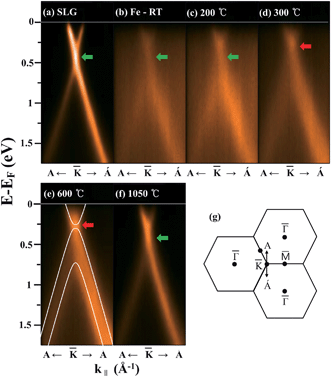
\includegraphics [scale=1] {arpes}
  \caption{Спектры фотоэлектронной спектроскопии с угловым разрешением, полученные при различных температурах отжига в работе \cite{C3NR04178F}}. 
  \label{img:arpes}  
\end{figure}

Альтернативным путем создания интерфейса графен/ферромагнетик является интеркаляция атомами металла графена, сформированного на карбиде кремния. Внедрение атомов железа в систему графен/SiC(0001) ранее исследовалось в работе \cite{C3NR04178F}, авторы которой установили, что при отжиге до температуры 600$^o$С атомы железа проникают под буферный слой, что подтверждается как экспериментальными данными, так и теоретическими расчетами. Так, из анализа фотоэлектронных спектров становится ясно, что при внедрении железа пропадают связи атомов буферного слоя с подложкой. Особый интерес представляет спектральная линия C $1s$, которая согласно данным работы \cite{PhysRevB.77.155303} включает в себя четыре компоненты. Наиболее интенсивная из них (мода G) соответствует графену. Вторая компонента (SiC) относится к атомам углерода в карбиде кремния. Наконец, моды S1 и S2 соответствуют двум типам атомов углерода в буферном слое, находящемся между графеном и верхним слоем атомов SiC(0001). При этом компонента S1 относится к тем атомам углерода, которые связаны висячими связями с нижележащим слоем SiC, а мода S2 соответствует атомам углерода, не связанным с этим слоем. После интеркаляции железа вклады всех мод, кроме G, значительно ослабляются (Рис. \ref{img:c1s}). 

Дополнительным свидетельством интеркаляции атомов железа под графен является отсутствие окисления полученного интерфейса после выдерживания в кислороде. Утверждается, что буферный слой отделяется от подложки, и на поверхности образуется двухслойный графен. Это должно приводить к возникновению характерных параболических дисперсионных кривых в окрестности точки К. Однако на спектрах фотоэлектронной спектроскопии с угловым разрешением видно, что после интеркаляции железа дисперсия $\pi$-состояний углерода лишь становится диффузной, размытой (Рис. \ref{img:arpes}).   



\section{ Выводы из обзора и постановка задач исследования} \label{chapt3}
Несмотря на растущий интерес исследователей к получению структур типа графен/ферромагнетик/диэлектрик, исследованию системы графен/Fe/SiC(0001) посвящена только работа \cite{C3NR04178F}. В ней показана возможность интеркалирования графена, выращенного на карбиде кремния, железом. При этом утверждается, что буферный слой при этом отрывается от подложки, и на поверхности интерфейса формируется квазисвободный двухслойный графен. Однако остается невыясненной локализация атомов железа в пленке. Кроме того, неясно, как интеркаляция атомов железа влияет на электронную структуру буферного слоя. В соответствии с литературными данными, в результате взаимодействия атомов буферного слоя и железа должны возникать гибридные орбитали, и, следовательно, буферный слой должен быть сильно связан с подложкой. Таким образом, ряд вопросов остается невыясненным. 

Целью настоящей диссертации стало получение новых знаний о системе графен/Fe/SiC(0001).

В соответствии с целью работы были поставлены следующие задачи:

1. изучение оптимальных условий формирования структуры графен/Fe/SiC(0001);

2. установление мест локализации атомов железа;

3. проведение первопринципных расчетов электронной структуры систем графен/SiC(0001) и графен/Fe/SiC(0001).


\chapter{Метод функционала плотности} \label{chapt4}

\section{Теоретические основы}
	Одним из самых распространенных инструментов для теоретического анализа систем графен/подложка является метод функционала плотности (density functional theory). Данный подход позволяет моделировать кристаллическое строение исследуемой системы, а также получать информацию о её электронном строении.
	
	Метод функционала плотности лежит в основе современных расчетов электронных свойств твердых тел лежит  Его появление дало серьезный толчок для квантовой химии и вычислительной физики сложных конденсированных систем.
	
	Как известно, квантовая механика дает способ расчета многоэлектронных систем. Однако решение уравнения Шредингера возможно лишь в самых простых случаях. Суть проблемы в том, что волновая функция зависит от 3N переменных, где N — число электронов. Поэтому использование многоэлектронной волновой функции для описания твердых тел оказывается невозможным. 

Идея метода функционала плотности состоит в том, чтобы заменить волновую функцию  электронной плотностью, зависящей лишь от трех пространственных переменных. Возможность такой замены была показана в работе Кона и Хоэнберга в 1964 году \cite{25}. В этой работе были доказаны две теоремы, устанавливающие соответствие между волновой функцией, электронной плотностью и внешним полем. 

Теорема I. Для любой системы взаимодействующих электронов, находящихся во внешнем потенциале  , потенциал  определяется однозначно (с точностью до несущественной константы) электронной плотностью основного состояния  .

	Теорема II. Существует универсальный функционал  электронной плотности, справедливый для любого внешнего потенциала  . Для некоторого вполне определенного внешнего потенциала   экстремум (минимум) полной энергии   достигается для электронной плотности основного состояния n(r).
	
	Эти теоремы имеют важное значение, но не дают практических методов для вычисления наблюдаемых величин. Вид функционала Кона-Хоэнберга может быть установлен только для невзаимодействующего электронного газа или для системы частиц, описываемых в приближении Томаса-Ферми. Практическое значение метод приобрел только после того, как Кон и Шэм предложили подход для вычисления функционала плотности \cite{26}.
	
	Идея состояла в том, чтобы заменить истинный функционал вспомогательным функционалом системы свободных частиц. Вспомогательный гамильтониан выбирается так, чтобы он имел обычную кинетическую энергию и локальный потенциал, ответственный за кулоновское взаимодействие, корреляцию и обмен. 
	
	Уравнение Кона-Шэма выглядит следующим образом:
 	\begin{equation}
  \label{eq:equation1}
 -\frac{1}{2}\triangledown^2\psi_i(r)+v_{KS}(r)\psi_i(r)=\epsilon_i\psi_i(r)
\end{equation}

Оно имеет вид одночастичного уравнения Шрёдингера для частицы, движущейся в самосогласованном потенциале Кона-Шэма:
		 	\begin{equation}
  \label{eq:equation2}
 v_{KS}(r)=v_{ext}(r)+v_H(r)+v_{xc}(r)
\end{equation}
 	\begin{equation}
  \label{eq:equation3}
v_H(r)=\int\frac{n(r)}{|r-r'|}dr'
\end{equation}
 	\begin{equation}
  \label{eq:equation4}
v_{xc}(r)=\frac{\delta E_{xc}}{\delta n(r)}
\end{equation}

Средняя плотность электронов определяется выражением:
 	\begin{equation}
  \label{eq:equation5}
n(r)=\sum_i|\psi_i(r)|^2
\end{equation}
где индекс j пробегает по всех состояниям, которые заполнены в соответствии с принципом Паули.
В случае проведения вычислений магнитных свойств твердых тел необходимо вводить отдельно плотности электронов для случая с s=+1/2 и s=-1/2.
 	\begin{equation}
  \label{eq:equation6}
n^\uparrow(r)=\sum_i|\psi^\uparrow_i(r)|^2, n^\downarrow(r)=\sum_i|\psi^\downarrow_i(r)|^2
\end{equation}

Энергия становится функционалом ${n^\downarrow(r)}$ и ${n^\uparrow(r)}$:
 	\begin{equation}
  \label{eq:equation7}
E_{KS}[n^\uparrow,n^\downarrow]=T_s+E_H+E_{ext}+E_{xc}[n^\uparrow,n^\downarrow]
\end{equation}
	
	Принято использовать вместо ${n^\downarrow(r)}$ и ${n^\uparrow(r)}$ полную электронную плотность и намагниченность:
 	\begin{equation}
  \label{eq:equation8}
n(r)=n^\uparrow(r)+n^\downarrow(r), m(r)=n^\uparrow(r)-n^\downarrow(r)
\end{equation}
	
	Тогда уравнения Кона-Шэма принимают вид:
\begin{equation}
  \label{eq:equation9}
  %\begin{align}
 (-\frac{1}{2}\triangledown^2+V_H+V_{ext}+V_{xc}+B_{xc})\psi_i^\uparrow(r)=\epsilon_i^\uparrow\psi_i^\uparrow(r) \\
(-\frac{1}{2}\triangledown^2+V_H+V_{ext}+V_{xc}+B_{xc})\psi_i^\downarrow(r)=\epsilon_i^\downarrow\psi_i^\downarrow(r)
%\end{align}
 \end{equation}
где ${V_{xc}=\frac{\delta E_{xc}[n,m]}{\delta n(r)}}$ ,${B_{xc}=\frac{\delta E_{xc}[n,m]}{\delta m(r)}}$.
	
	Магнетизм исходит из обменно-корреляционного функционала: одно направление спина оказывается энергетически более выгодно, чем другое.
	Уравнения Кона-Шэма могут рассматриваться как формальное обобщение теории Хартри. Если бы было известно выражение для обменно-корреляционной энергии, было бы возможно точное описание многоэлектронных систем. Оказалось, что можно найти для обменно-корреляционной энергии удачную аппроксимацию. Наиболее простая – аппроксимация локальной плотности (local density approximation - LDA).
 	\begin{equation}
  \label{eq:equation10}
E_{xc}^{LDA}=\int drv_{xc}(n(r))n(r)
\end{equation}
где ${v_{xc}(n(r))}$ - обменно-корреляционная энергия на одну частицу однородного газа.
	
	Существует несколько подходов к усовершенствованию приближения локальной плотности. В одном из них построена теория, которая учитывает неоднородное распределение электронной плотности. Это обобщенно-градиентное разложение (generalized gradient approximation — GGA). Здесь выражение для обменно-корреляционной энергии раскладывается по степеням градиента плотности.
 	\begin{equation}
  \label{eq:equation11}
E_{xc}^{GGA}=\int drf(n(r),|\triangledown n(r)|)n(r)
\end{equation}
где ${f(n(r),|\triangledown n(r)|)}$ - некая функция, для которой получено приближенное выражение. Аналогичные уравнения можно написать для спин-поляризованного обобщенно-градиентного приближения.

	Рассмотрим теперь способ решения уравнений Кона-Шэма. Он является итерационным:

1.	На первом этапе задаются начальные приближения для электронной плотности $n(r)$;

2.	Затем вычисляется потенциал:
 	\[
v_{KS}(r)=v_H+v_{ext}(r)+v_{xc}(r), v_H=\int dr'\frac{n(r)}{|r-r'|}
\]		

3.	На следующем шаге решаются уравнения Кона-Шэма:


\[
 % \begin{align}
 (-\frac{1}{2}\triangledown^2+V_H+V_{ext}+V_{xc}+B_{xc})\psi_i^\uparrow(r)=\epsilon_i^\uparrow\psi_i^\uparrow(r) \\
(-\frac{1}{2}\triangledown^2+V_H+V_{ext}+V_{xc}+B_{xc})\psi_i^\downarrow(r)=\epsilon_i^\downarrow\psi_i^\downarrow(r)
  %\end{align}
 \]



4.	После этого находятся уточненные значения электронной плотности:
\[
n^\uparrow(r)=\sum_i|\psi^\uparrow_i(r)|^2, n^\downarrow(r)=\sum_i|\psi^\downarrow_i(r)|^2
\]
    
    Затем процедура повторяется, пока не будут выполнены критерии сходимости.
    
\section{Практическое применение}
	
	Теперь опишем некоторые практические аспекты решения уравнений Кона-Шема. При численном решении уравнений на собственные числа возникает необходимость в разложении волновых функций в базис. Базисными функциями могут быть как плоские волны, так и наборы локализованных функций (например, гауссовых). Широкое распространение получило использование в качестве базисных функций плоских волн. Их преимущества состоят в том, что они удобны для программирования, ортогональны друг другу и не зависят от позиций атомов. С другой стороны, для корректного представления волновых функций требуется большое число базисных функций (в общем случае — бесконечность). Другой недостаток плоских волн связан с тем, что набор функций в наборе дискретен только в случае периодической системы.
	
	Для волновой функции электрона в периодическом потенциале справедлива теорема Блоха
 	\begin{equation}
  \label{eq:equation12}
\psi_k(r)=e^{ikr}u_k(r)
\end{equation}
где u(k) — периодическая функция, то есть
 	\begin{equation}
  \label{eq:equation13}
u(r)=u(r+R)
\end{equation}
где R — вектор трансляции. В Фурье-разложении такой функции возникают только определенные плоские  волны:
 	\begin{equation}
  \label{eq:equation14}
u_k(r)=\frac{1}{\Omega}\sum_Gc_{k,G}e^{iGr}
\end{equation}
где G — вектор трансляции в обратном пространстве, причем плоские волны, которые появляются в таком разложении, можно представить как сетку в обратном пространстве, причем эта сетка простирается на бесконечность и является дискретной только для периодических систем.  Однако на практике оказывается, что вклады высоких гармоник в разложение пренебрежимо малы. Следовательно, можно ограничить набор теми плоскими волнами, для которых
 	\begin{equation}
  \label{eq:equation15}
\frac{h^2|k+G|^2}{2m_e}\le E_{cut}
\end{equation}
где   — энергия обрезки. Её значение подбирают таким образом, чтобы точность вычислений была приемлемой при как можно меньшем размере базиса.
	
	Уравнения Кона-Шема в базисе плоских волн выглядят следующим образом:
 	\begin{equation}
  \label{eq:equation16}
\sum_GH_{k+G,k+G'}c_{i,k+G}=\epsilon_ic_{i,k+G}
\end{equation}
где матричный элемент Гамильтониана дается формулой:
 	\begin{equation}
  \label{eq:equation17}
\frac{1}{2}|k+G|^2\delta_{G,G'}+V_{ion}(k+G,k+G')+V_H(G-G')+V_{xc}(G+G')
\end{equation}
	
	Рассмотрим слагаемое, связанное с потенциалом ядер. Ядро создает вокруг себя кулоновский потенциал, который выражается простой и известной формулой: 
 	\begin{equation}
  \label{eq:equation18}
V_{nuc}=-\frac{z}{r}
\end{equation}

Однако такая форма потенциала является причиной вычислительных затруднений.  Электроны в атоме можно условно разделить на две группы. К первой группе относятся остовные электроны, локализованные в окрестности ядра и не участвующие в формировании химических связей. Их волновые функции имеют резкие пики вблизи ядра. Ко второй группе принадлежат валентные электроны. Их волновые функции имеют максимумы вдали от ядра и в окрестности ядра осциллируют из-за требования ортогональности.  При образовании связей волновые функции валентных электронов могут значительно перестраиваться. Наличие вблизи ядра острых максимумов волновых функций остовных электронов и осцилляций волновых функций валентных электронов обуславливает появление в Фурье-разложении высоких гармоник, что приводит к большим энергиям отсечки. Решением этой проблемы является введение псевдопотенциала. В методе псевдопотенциала волновые функции остовных электронов заменяются псевдофункциями, гладкими вблизи ядра и совпадающими с «честными» волновыми функциями вдали от него. Таким образом, кулоновский потенциал ядер становится экранированным. Уравнения Кона-Шема теперь решаются только для валентных электронов, которые участвуют в формировании химических связей. Помимо снижения вычислительной затратности за счет учета только валентных электронов, использование псевдопотенциала приводит в уменьшению числа функций базиса за счет исчезновения осцилляций волновых функций в окрестности ядра и, следовательно, уменьшения энергии обрезки.
	
	Все вышесказанное применимо к периодическим системам, таким как объемные кристаллы. Однако на практике исследуемая система часто представляет собой тонкую пленку, квантовую нить, квантовую точку или отдельную молекулу. В этом случае удобно выбирать для трансляции суперячейку, содержащую вакуумные зазоры в направлениях, в которых отсутствует периодичность. Ширина зазоров выбирается таким образом, чтобы соседние структуры не влияли друг на друга. Такой подход обеспечивает дискретный набор базисных волновых функций и позволяет рассчитывать свойства систем пониженной размерности.

Метод функционала плотности получил широкое распространение и в настоящий момент является одним из самых популярных инструментов для расчетов свойств твердых тел и наноразмерных систем.


\chapter{Техника эксперимента} \label{chapt_exp_tech}
\section{Дифракция медленных электронов} \label{leed}
Дифракция медленных электронов (ДМЭ) позволяет исследовать структуру поверхностных слоев кристаллов.  В настоящей работе ДМЭ использовалась для определения взаимного расположения графена и подложки, а также для контроля качества исследуемой системы. На Рис. \ref{img:leed_scheme} показана экспериментальная реализация данного метода. Основные части установки - это электронная пушка, набор металлических сеток, держатель образца и флюоресцентный экран. В ходе измерения образец помещается в центр полусферы, электроны эмитируются катодом электронной пушки, разгоняются до необходимой энергии (20-200 эВ), движутся в бесполевом пространстве по направлению к образцу и рассеиваются на его приповерхностных слоях. Тормозящие сетки отсекают неупруго рассеянные электроны. Пучки упруго рассеянных электронов, прошедшие сетки, ускоряются до энергий 5-7 кэВ и попадают на флюоресцентный экран, после чего на нем наблюдают дифракционную картину. 
Для исследования атомной структуры приповерхностных слоев энергия первичных электронов должна удовлетворять условию наблюдения дифракционной картины: длина волны электрона $\lambda$ должна быть сравнима с расстояниями между атомами. Длина волны де-Бройля для электронов определяется из соотношений
 	\begin{equation}
  \label{eq:equation1}
 \lambda=\frac{h}{p}=\frac{h}{\sqrt{2mE}}, \lambda[\buildrel _\circ \over {\mathrm{A}}]\approx\frac{150}{E[eV]}.
\end{equation}
Высокая поверхностная чувствительность метода ДМЭ определяется тем, что при таких энергиях длина свободного пробега электрона составляет несколько атомных слоев, и поэтому большинство актов упругого рассеяния происходит в верхних слоях кристалла.
 \begin{figure}[ht] 
  \center
  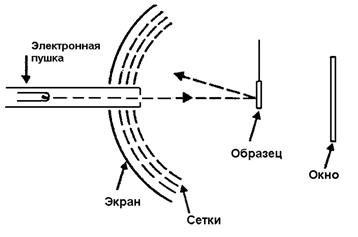
\includegraphics [scale=1] {./Dissertation/images/leed_scheme.jpg}
  \caption{Схема стандартного эксперимента по ДМЭ.} 
  \label{img:leed_scheme}  
\end{figure}
 

Пусть $\overrightarrow{k}$ и $\overrightarrow{k'}$ — волновые векторы падающей и рассеянной электронной волны. Представим их в виде суммы двух компонент, одна из которых параллельна плоскости поверхности, а другая ей перпендикулярна: $\overrightarrow{k}=\overrightarrow{k_\perp}+\overrightarrow{k_\parallel}$ (аналогично для $\overrightarrow{k'}$). Для квазидвумерных систем, когда периодичность структуры наблюдается только в плоскости параллельной поверхности, при рассеянии электронной волны сохраняется лишь компонента волнового вектора $k_\parallel$ (с добавлением вектора обратной решётки $\overrightarrow{g_{h_k}}$.На основании законов сохранения энергии и импульса справедливы следующие соотношения:
 	\begin{equation}
  \label{eq:equation100}
\overrightarrow{k}=\overrightarrow{k'}
\end{equation}
или
 	\begin{equation}
  \label{eq:equation1}
\overrightarrow{k_\parallel}+\overrightarrow{k_\perp}=\overrightarrow{k'_\parallel}+\overrightarrow{k'_\perp}
\end{equation}
 	\begin{equation}
  \label{eq:bragg}
\overrightarrow{k'_\parallel}=\overrightarrow{k_\parallel}+\overrightarrow{g_{h_k}},  \overrightarrow{g_{h_k}}=h\overrightarrow{a^*}+k\overrightarrow{b^*}.
\end{equation}


Базисные векторы трансляции обратной решётки $\overrightarrow{a^*}$и $\overrightarrow{b^*}$ связаны с векторами решётки в прямом пространстве $\overrightarrow{a}$ и $\overrightarrow{b}$ соотношениями

 	\begin{equation}
  \label{eq:equation1}
\overrightarrow{a^*}=\frac{\overrightarrow{b}\times\overrightarrow{n}}{A},  \overrightarrow{b^*}=\frac{\overrightarrow{n}\times\overrightarrow{a}}{A},  A=\overrightarrow{a}\cdot\overrightarrow{b}\times\overrightarrow{n}.
\end{equation}

где $\overrightarrow{n}$ — единичный вектор нормали к поверхности.
Выражения (\ref{eq:equation100}–\ref{eq:bragg}), представляют собой закон Брэгга,
описывающий условия конструктивной интерференции падающей и рассеянной волны. Таким образом, дифрагированным пучкам соответствуют индексы обратной решётки ($hk$) (в трёхмерном случае — $hkl$). По их расположению можно сделать вывод о симметрии обратной решётки, а значит, используя уравнения (\ref{eq:bragg}), и о структуре решётки в прямом пространстве.
\section{Фотоэлектронная спектроскопия остовных уровней}
Фотоэлектронная спектроскопия (ФЭС) является мощным инструментом для исследования поверхности твердых тел.

В данном методе исследуемый образец подвергается воздействию рентгеновского или ультрафиолетового излучения. Затем спектр фотовозбужденных электронов регистрируется с высоким энергетическим разрешением. Существует две разновидности ФЭС. В одном варианте регистрируются и анализируются спектры фотоэлектронов, эмитированных при возбуждении остовных уровней, в другом исследуются спектры электронов валентной зоны. В первом случае спектр является дискретным, причем каждая его линия характеризует возбуждение фотоэлектронов с определенных атомных уровней. Энергии связи остовных электронов специфичны для разных элементов, следовательно, можно установить, из каких элементов состоит приповерхностная область образца. Кроме того, величина энергии связи зависит от химического окружения атома, и поэтому измерение положения остовных уровней используется для определения химических соединений. Анализ таких энергетических сдвигов стал возможным благодаря появлению мощных источников синхротронного излучения. Они значительно расширили возможности метода спектроскопии остовных уровней, превратив его в эффективный метод исследования поверхности твердого тела. 

Рассмотрим физические основы метода. Диаграмма, иллюстрирующая процесс фотоэмиссии остовного электрона, показана в левой части Рис. \ref{img:pes}. Энергия связи $E_i$ остовного электрона в твердом теле отсчитывается относительно уровня Ферми, а не относительно уровня вакуума как в свободном атоме. Поэтому кинетическая энергия электрона ($E$), возбужденного с $i$-го уровня фотоном с энергией $h\nu$, равна: 
 	\begin{equation}
  \label{eq:equation101}
E=h\nu-E_i -e\phi,
\end{equation}
где $e\phi$ – это работа выхода материала, а величина $Е$ рассчитывается относительно уровня вакуума.

Из этой формулы видно, что энергия связи $E_i$ остовного фотоэлектрона определяется только его кинетической энергией при заданной величине $h\nu$ и известном значении $e\phi$. В экспериментальных условиях, кроме того, возникает контактная разность потенциалов $U_c$ между эмиттером и спектрометром, которая влияет на энергию возбужденных электронов, и изменяет ее значение на величину $еU_c$. Данная величина определяется как разница между работой выхода материала образца и работой выхода материала спектрометра ($U_s$). Принимая во внимание данный фактор, из формулы \ref{eq:equation101} получается следующее выражение для расчета энергии связи остовного фотоэлектрона:
 	\begin{equation}
  \label{eq:equation102}
E=h\nu-E_{kin} -e\phi_s,
\end{equation}
где $E_{kin}$ – измеряемое значение кинетической энергии фотоэлектрона (см. \ref{img:pes}).

 \begin{figure}[ht] 
  \center
  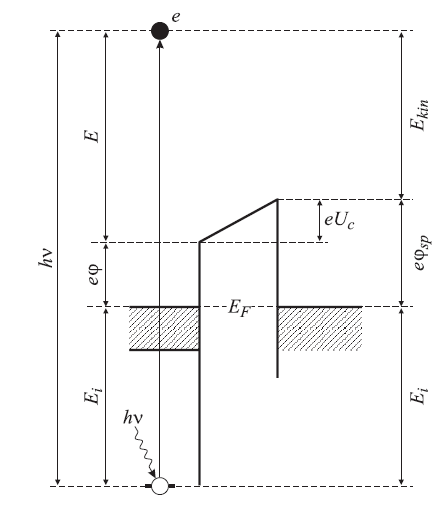
\includegraphics [scale=0.47] {./Dissertation/images/pes.png}
  \caption{Схематическая диаграмма, иллюстрирующая процесс возбуждения остовного электрона.} 
  \label{img:pes}  
\end{figure}


Таким образом, для того, чтобы определить энергию связи фотоэлектрона, нет необходимости знать работу выхода исследуемого образца. Требуется только рассчитать значение $e\phi_s$, которое находят при калибровке спектрометра с использованием эталонного образца. Легко видеть, что в случае металла энергия связи остовного электрона может быть также определена из сопоставления его кинетической энергии и кинетической энергии возбужденного с уровня Ферми металла валентного электрона. 
В рамках представленной на Рис. \ref{img:pes} модели, предполагается, что электроны, выходя из образца, не испытывают неупругих потерь энергии. Это происходит, если фотоэлектроны возбуждаются в относительно тонком приповерхностном слое толщиной меньшей, чем средняя длина свободного пробега ($\lambda$) до момента неупругого рассеяния. Величина длины свободного пробега зависит от энергии электрона, а эта зависимость имеет сходный вид для всех материалов (Рис. \ref{img:pes2}) с минимумом в области энергий порядка нескольких десятков эВ.
 \begin{figure}[ht] 
  \center
  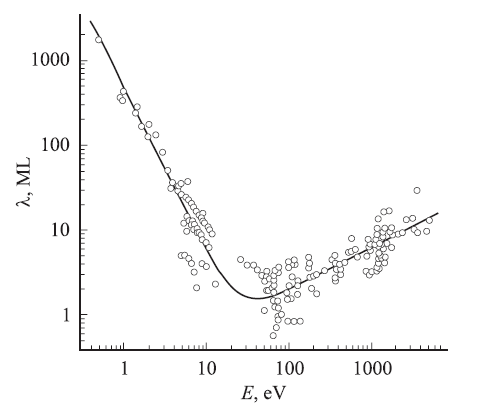
\includegraphics [scale=0.67] {./Dissertation/images/pes2.png}
  \caption{Зависимость средней длины свободного пробега электрона от энергии.} 
  \label{img:pes2}  
\end{figure}
 

Если глубина выхода фотоэлектрона без потерь энергии значительно превышает толщину приповерхностного слоя, то главный вклад в линию спектра вносят фотоэлектроны, эмитируемые атомами из объема, а спектр при этом называется объемно-чувствительным. Если же эти параметры имеют сопоставимые величины, то электроны, испускаемые атомами приповерхностной области, вносят значительный вклад в линию спектра, и такой спектр является поверхностно-чувствительным. Ясно, что для того, чтобы спектр был наиболее чувствительным к состоянию поверхности, энергии фотоэлектронов должны соответствовать минимуму зависимости $\lambda$(Е). Как правило, этого можно достигнуть выбором энергии фотонов. Объемно-чувствительный спектр принято измерять при энергиях, которые находятся на ниспадающей части зависимости $\lambda$(Е), где величина $\lambda$ сильно понижается при увеличении энергии. В таком случае для того, чтобы перейти от объемно-чувствительного спектра к поверхностно-чувствительному, достаточно понизить энергию фотонов лишь на несколько десятков электрон-вольт. Чтобы дополнительно усилить вклад приповерхностной области в спектре, необходимо увеличить полярный угол вылета исследуемых фотоэлектронов. Чем больше значение этого угла (отсчитываемое от нормали к поверхности), тем меньше глубина выхода электронов, и тем более значительный вклад в общий спектр дают поверхностные атомы. 
Как уже было отмечено, для практической реализации метода требуется применение синхротронного источника излучения, который имеет высокую плотность потока фотонов, а также дает возможность изменять их энергию. Кроме того, требуется наличие электронного спектрометра, обладающего достаточно высоким энергетическим разрешением.
Необходимо также отметить, что спектры остовных уровней обычно приводят в виде зависимости интенсивности фотоэлектронов от энергии связи. При этом за ноль шкалы энергий принимают либо энергию на уровне Ферми изучаемого образца, либо энергию связи электронов из атомов объема. Во втором случае атомы поверхности, остовные уровни которых имеют бóльшую энергию связи, чем атомы объема, имеют положительный энергетический сдвиг. Как правило, при этом приводят лишь узкий участок спектра вблизи выбранной линии.

\section{ Фотоэлектронная спектроскопия с угловым разрешением}  \label{chapt3}
ФЭСУР является основным методом для получения дисперсионных зависимостей $E(\overrightarrow{k})$ электронных состояний валентной зоны кристаллов. Для исследований зонной структуры методом ФЭСУР обычно выбирают такие энергии фотонов, при которых происходит прямой переход электрона в возбуждённое состояние, т.е. изменение энергии фотоэлектрона происходит при сохранении его импульса. Иными словами, импульс фотона должен быть пренебрежимо мал по сравнению с размерами зоны Бриллюэна кристалла. С другой стороны, энергию фотонов не следует выбирать слишком маленькой, чтобы конечное состояние возбуждённого электрона описывалось уже не блоховской волновой функцией, а плоской волной с параболическим законом дисперсии, иначе вместо плотности начальных состояний придётся иметь дело с приведённой плотностью начальных и конечных состояний.
При фотовозбуждении происходит прямой переход электрона из состояния в валентной зоне с квазиимпульсом $k_i$, описываемого блоховской функцией, в состояние плоской волны с импульсом $k_f$, при этом $k_f=k_i$.  Удобно разложить векторы импульса фотоэлектрона до (индекс $in$) и после ($out$) выхода из кристалла в вакуум на составляющие, параллельные ($\parallel$) и перпендикулярные ($\perp$) плоскости поверхности:
 	\begin{equation}
  \label{eq:arpes2}
k_f=k^{in}_\parallel+k^{in}_\perp, k^{out}=k^{out}_\parallel+k^{out}_\perp
\end{equation}

Поскольку при переходе через поверхность электрон теряет часть своей энергии (на величину работы выхода), перпендикулярная составляющая им
пульса $k^{in}_\perp$ уменьшается, при этом параллельная компонента $k^{in}_\parallel$ сохраняется с точностью до вектора обратной решётки кристалла $G$: $k^{out}_\parallel=k^{in}_\parallel+G$. Если рассматривать только первую зону Бриллюэна, т.е. работать в приведённой зонной схеме, можно считать $k^{out}_\parallel=k^{in}_\parallel$ . При выходе электрона в вакуум происходит изменение направления его движения. Зная угол $\theta$ и измеряя кинетическую энергию движущегося в вакууме в данном направлении фотоэлектрона, можно получить следующее выражение для $k^{in}_\parallel$:
\begin{equation}
\label{eq:arpes}
k^{in}_\parallel=k^{out}_\parallel sin\theta=\sqrt{\frac{2m}{h^2}E_{kin}}sin\theta
\end{equation}
Выражение \ref{eq:arpes} является основным в методе ФЭСУР. Меняя полярный угол $\theta$ и измеряя ФЭ спектр, можно получить набор данных $E^{in}_B(k_\parallel)$, т.е. дисперсионную зависимость в спроецированной на поверхность зоне Бриллюэна вдоль направления, задаваемого азимутальным углом $\phi$. Для двумерных систем, таких как графен, этого достаточно для построения полной картины дисперсии зон, потому что зона Бриллюэна двумерна. В случае же трёхмерных систем ситуация более сложная, так как для определения зависимости $E^{in}_B(k_\perp)$ необходимо получить спектры при разных энергиях фотонов.
 Пучок фотонов, попадая на образец, вызывает эмиссию первичных и вторичных электронов, распределение по энергии и углам которых регистрируется с помощью полусферического анализатора. Поскольку данный метод требует измерений зависимости энергетического спектра фотоэлектронов от направления их движения $\theta$, высокое угловое разрешение анализатора является одним из самых важных условий.

\section{ Ближняя тонкая структура рентгеновских спектров поглощения}
Спектроскопия поглощения рентгеновского излучения основана на измерении зависимости коэффициента поглощения излучения от энергии фотонов. Примерный вид такой зависимости приведён на Рис. \ref{img:nexafs}. Её характерными особенностями являются: (i) наличие резких скачков в коэффициенте поглощения при определённых энергиях, называемых краями поглощения; (ii) за этими краями наблюдается убывание коэффициента поглощения; (iii) чуть выше краёв видна так называемая тонкая структура, модулирующая коэффициент поглощения. Каждый край связан с переходом электрона с внутреннего уровня определённого атома в незаполненные состояния. Исследование ближней тонкой структуры рентгеновских спектров поглощения (БТСРСП, англ. NEXAFS) является широко распространённым методом изучения кристаллической и электронной структуры незаполненных состояний твёрдых тел (или молекул), поскольку оказывается очень чувствительным к электронному состоянию поглощающего атома и его окружению [165].
 \begin{figure}[ht] 
  \center
  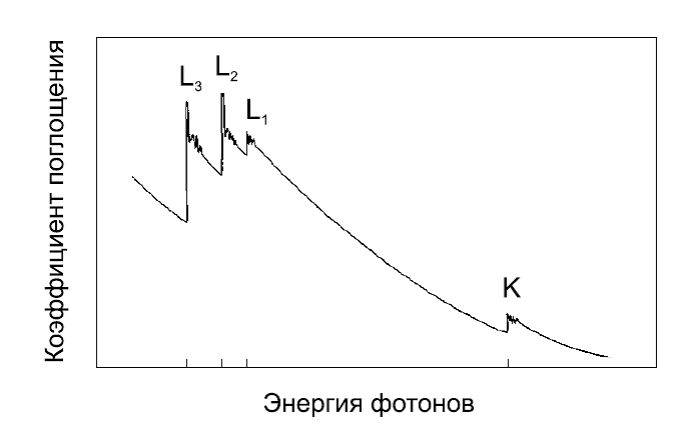
\includegraphics [scale=0.47] {./Dissertation/images/nexafs.png}
  \caption{Характерная зависимость коэффициента поглощения рентгеновского излучения от
энергии фотонов [164].} 
  \label{img:nexafs}  
\end{figure}
Для слоистых систем с $sp^2$ гибридизацией метод исследования БТСРСП позволяет получить информацию не только об интегральной плотности свободных состояний, но также выделить вклад в электронную структуру $\pi$ и $\sigma$ орбиталей, а также определить их ориентацию относительно плоскости поверхности образца. Для этого используется излучение с линейной поляризацией. Спектры поглощения снимаются при разных углах падения излучения на образец, и в зависимости от угла между направлением связи и вектором поляризации изменяется вероятность возбуждения электронов в состояния различной направленности. Так, если $\sigma$ связи находятся в плоскости поверхности образца, а $\pi$ перпендикулярны ей, то интенсивность переходов в $\sigma^*$ состояния будет максимальна при падении излучения по нормали к образцу, поскольку в этом случае вектор поляризации будет направлен вдоль $\sigma$ связей. Вероятность перехода в $\pi^*$ состояния при этом будет нулевой. Ситуация поменяется на противоположную, если направить линейно поляризованное излучение по касательной к поверхности образца.
Для изучения БТСРСП необходим источник излучения, позволяющий варьировать энергию фотонов с достаточно малым шагом, поскольку важная информация может содержаться в незначительном изменении энергетическо го положения (< 0.2 эВ), относительной интенсивности или расщеплении пиков тонкой структуры. Эксперименты по исследованию БТС проводятся с использованием синхротронного излучения. Каналы вывода синхротронного
излучения из накопителя в экспериментальную камеру содержат множество оптических элементов, например, фокусирующие зеркала и решётки монохроматора.
\section{ Экспериментальная станция}
 \begin{figure}[ht] 
  \center
  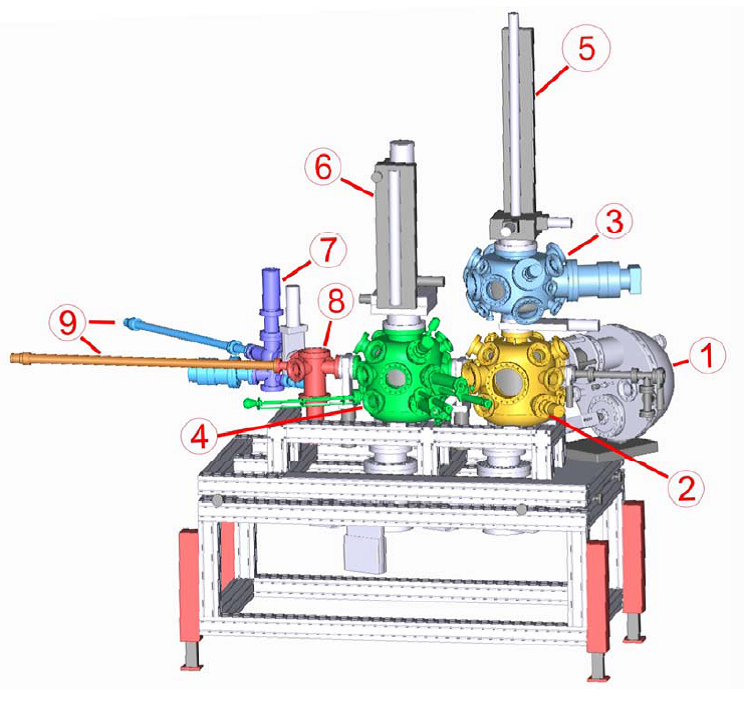
\includegraphics [scale=0.47] {./Dissertation/images/station.png}
  \caption{Изображение станции RGBL на синхротроне BESSY II: 1 - полусферический анализатор, 2 - аналитическая камера, 3, 4 - препарационные камеры, 5, 6 - стойки вертикального перемещения образцов, 7 - загрузочная камера, 8 - камера замены образцов, 9 - система горизонтального перемещения образцов.} 
  \label{img:bessy}  
\end{figure}
Результаты экспериментов, описанные в настоящей работе, получены в Российско-Германской лаборатории на синхротроне BESSY II. Схема экспериментальной станции показана на Рис. \ref{img:bessy}. Две основных части станции - препарационная и аналитическая камеры. В препарационной камере проводился отжиг образца, контроль его струкутуры методом ДМЭ и напыление железа. В аналитической камере проводились измерения спектров XPS и NEXAFS. Помимо этого на станции есть камеры загрузки и замены образцов, а также система их перемещения.

Спектры фотоэлектронной спектроскопии были получены с одного из образцов позже на станции Нанофэс синхротрона Курчатовского института.


\chapter*{Заключение}                       % Заголовок
\addcontentsline{toc}{chapter}{Заключение}  % Добавляем его в оглавление

%% Согласно ГОСТ Р 7.0.11-2011:
%% 5.3.3 В заключении диссертации излагают итоги выполненного исследования, рекомендации, перспективы дальнейшей разработки темы.
%% 9.2.3 В заключении автореферата диссертации излагают итоги данного исследования, рекомендации и перспективы дальнейшей разработки темы.
%% Поэтому имеет смысл сделать эту часть общей и загрузить из одного файла в автореферат и в диссертацию:

Основные результаты работы заключаются в следующем.
\input{common/concl}

      % Заключение
\include{Dissertation/acronyms}        % Список сокращений и условных обозначений
\include{Dissertation/dictionary}      % Словарь терминов
\include{Dissertation/references}      % Список литературы
\include{Dissertation/lists}           % Списки таблиц и изображений (иллюстративный материал)

\setcounter{totalchapter}{\value{chapter}} % Подсчёт количества глав

%%% Настройки для приложений
\appendix
% Оформление заголовков приложений ближе к ГОСТ:
\setlength{\midchapskip}{20pt}
\renewcommand*{\afterchapternum}{\par\nobreak\vskip \midchapskip}
\renewcommand\thechapter{\Asbuk{chapter}} % Чтобы приложения русскими буквами нумеровались

%\include{Dissertation/appendix}        % Приложения

\setcounter{totalappendix}{\value{chapter}} % Подсчёт количества приложений

\end{document}
